\documentclass[12pt]{article}

% Packages
\usepackage[margin=1in]{geometry}
\usepackage{fancyhdr}
\usepackage{amsmath, amsthm, amssymb, physics}
\usepackage{dirtree, graphicx}

% Page Style
\fancypagestyle{plain}{
    \fancyhf{}
    \renewcommand{\headrulewidth}{0pt}
    \renewcommand{\footrulewidth}{0pt}
    \fancyfoot[R]{\thepage}
}
\pagestyle{plain}

% Problem Box
\setlength{\fboxsep}{4pt}
\newsavebox{\savefullbox}
\newenvironment{fullbox}{\begin{lrbox}{\savefullbox}\begin{minipage}{\dimexpr\textwidth-2\fboxsep\relax}}{\end{minipage}\end{lrbox}\begin{center}\framebox[\textwidth]{\usebox{\savefullbox}}\end{center}}
\newenvironment{pbox}[1][]{\begin{fullbox}\ifx#1\empty\else\paragraph{#1}\fi}{\end{fullbox}}

% Options
\renewcommand{\thesubsection}{\thesection(\alph{subsection})}
\allowdisplaybreaks
\addtolength{\jot}{4pt}
\theoremstyle{definition}
\setlength{\parindent}{0pt}

% Default Commands
\newtheorem{proposition}{Proposition}
\newtheorem{lemma}{Lemma}
\newcommand{\ds}{\displaystyle}
\newcommand{\isp}[1]{\quad\text{#1}\quad}
\newcommand{\N}{\mathbb{N}}
\newcommand{\Z}{\mathbb{Z}}
\newcommand{\Q}{\mathbb{Q}}
\newcommand{\R}{\mathbb{R}}
\newcommand{\C}{\mathbb{C}}
\newcommand{\eps}{\varepsilon}
\renewcommand{\phi}{\varphi}
\renewcommand{\emptyset}{\varnothing}
\newcommand{\pfrac}[2]{\left(\frac{#1}{#2}\right)}

% Extra Commands


% Document Info
\fancypagestyle{title}{
    \renewcommand{\headrulewidth}{0.4pt}
    \setlength{\headheight}{15pt}
    \fancyhead[R]{Harry Coleman}
    \fancyhead[L]{GEOG 191 Assignment 8}
    \fancyhead[C]{March 1, 2021}
}

% Begin Document
\begin{document}
\thispagestyle{title}


\begin{pbox}[4]
    Solve using the branch and bound method.
    \[\begin{array}{ll}
        \textbf{Maximize} & z = 5x_1 + 2x_2 - 7x_3 \\
        \textbf{Subject to}
            & x_2 + 4x_3 \leq 13 \\
            & 4x_1 - 2x_2 \leq 12 \\
            & x_1, x_2, x_3 \geq 0 \\
            & x_1, x_2 \text{ integer}
    \end{array}\]
\end{pbox}


The notation $x = (x_1, x_2, x_3)$ is used for solutions. We obtain the following branch and bound tree.

\vspace{1em}
\dirtree{%
.1 Initial: $z=73.5$ at $x = (9.5, 13, 0)$.
.2 $x_1 \leq 9$: $z = 71$ at $x = (9, 13, 0)$.
.2 $x_1 \geq 10$: infeasible (fathom).
}
\vspace{1em}

Hence, we have an optimal solution of $x = (9, 13, 0)$ with objective $z = 71$. The following code was used.
\begin{center}
    \begin{minipage}{0.3\textwidth}
        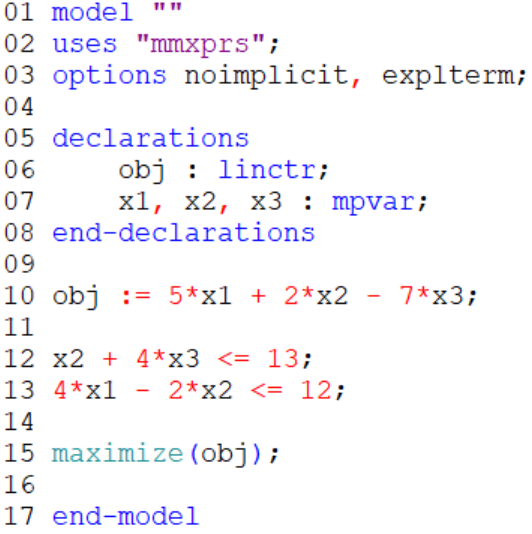
\includegraphics[width=\textwidth]{code1a.png}
    \end{minipage}
    \begin{minipage}{0.3\textwidth}
        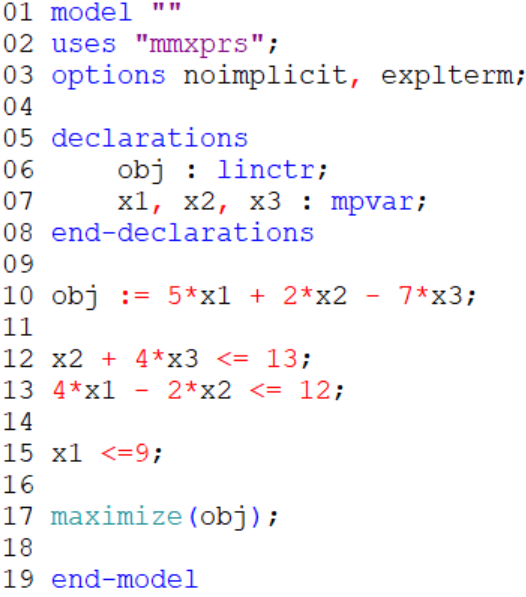
\includegraphics[width=\textwidth]{code1b.png}
    \end{minipage}
    \begin{minipage}{0.3\textwidth}
        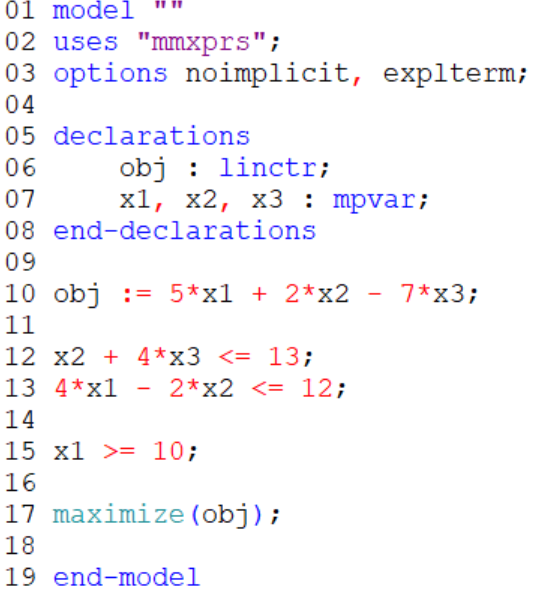
\includegraphics[width=\textwidth]{code1c.png}
    \end{minipage}
\end{center}



\newpage
\begin{pbox}[5]
    Solve using the branch and bound method.
    \[\begin{array}{ll}
        \textbf{Maximize} & z = 4x_1 - 7x_2 \\
        \textbf{Subject to}
            & -x_1 + x_2 \geq 5 \\
            & 4x_1 + 3x_2 \geq 17 \\
            & x_1, x_2 \geq 0 \\
            & x_1, x_2 \text{ integer}
    \end{array}\]
\end{pbox}

The original problem was a minimization, which is unbounded by making $x_2$ arbitrarily large, so I am assuming maximization was intended. We obtain the following branch and bound tree.

\vspace{1em}
\dirtree{%
.1 Initial: $z=-35.9571$ at $x = (0.2857, 5.2857)$.
.2 $x_1 \leq 0$: $z = -39.6667$ at $x = (0, 5.6667)$ worse bound (fathom).
.2 $x_1 \geq 1$: $z = -38$ at $x = (1, 6)$.
}
\vspace{1em}

Hence, we have an optimal solution of $x = (1, 6)$ with objective $z = -38$. The following code was used.
\begin{center}
    \begin{minipage}{0.3\textwidth}
        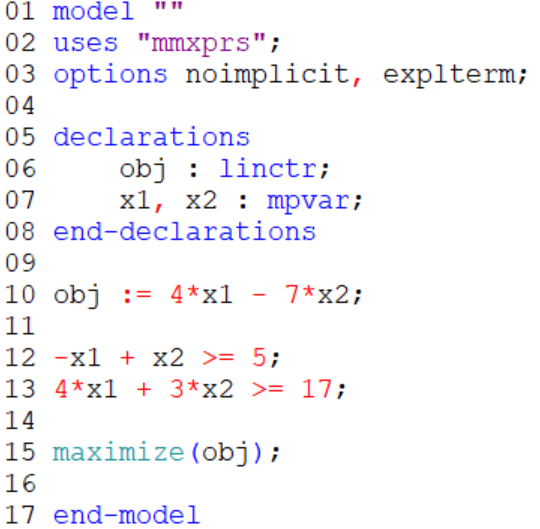
\includegraphics[width=\textwidth]{code2a.png}
    \end{minipage}
    \begin{minipage}{0.3\textwidth}
        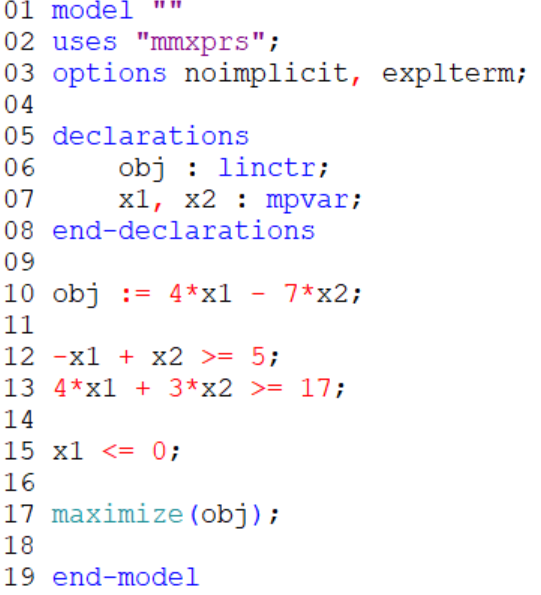
\includegraphics[width=\textwidth]{code2b.png}
    \end{minipage}
    \begin{minipage}{0.3\textwidth}
        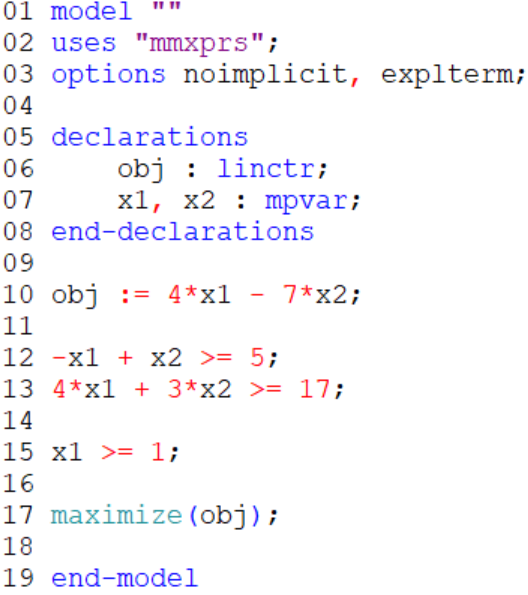
\includegraphics[width=\textwidth]{code2c.png}
    \end{minipage}
\end{center}

\end{document}